\chapter{Open Problems and the Bridge to Hilbert's Eighth Problem}
\label{ch:open}

\section{Two problems about the heat equation}

Hilbert's eighth problem contains the Riemann hypothesis. It appears in a list about prime numbers, far from the axioms of physics, and the two problems are usually treated as belonging to different worlds. This chapter points to a common mathematical structure. The Riemann hypothesis is equivalent to a statement about the backward flow of the heat equation, and the inferential form of the sixth problem, which asks to recover the initial state of a dissipative system from later observations, is a backward problem for a parabolic equation. This is an analogy and not an equivalence. Both have probabilistic formulations in terms of Brownian motion, and the eighth problem has a natural expression in the language of ferromagnetic random variables that Lee, Yang and Newman developed for statistical mechanics.

\section{The de Bruijn Newman constant}

Let $\xi(s) = \frac12s(s-1)\pi^{-s/2}\Gamma(s/2)\zeta(s)$ and $\Xi(x) = \xi(\frac12+ix)$. Riemann's representation of $\Xi$ as a Fourier transform~\cite{riemann1859}, which P\'olya wrote with an explicit kernel~\cite{polya1926}, reads in the scaling of Rodgers and Tao~\cite{rodgerstao2020}
\begin{gather*}
\Xi(x) = 8\int_0^\infty\Phi(u)\cos(2xu)\dd u, \\
\Phi(u) = \sum_{n=1}^\infty\big(2\pi^2n^4e^{9u}-3\pi n^2e^{5u}\big)\exp\big(-\pi n^2e^{4u}\big),
\end{gather*}
where $\Phi$ is even in $u$ when extended to the line, positive, rapidly decreasing, and decreasing on $(0,\infty)$. The Riemann hypothesis is the statement that all zeros of $\Xi$ are real. Following de Bruijn~\cite{debruijn1950} and Newman~\cite{newman1976}, define for $t\in\R$
\[
H_t(z) = \int_0^\infty e^{tu^2}\Phi(u)\cos(zu)\dd u,
\]
so that $H_0(z) = \frac18\Xi(z/2)$, whose zeros are at $\pm2\gamma_n$ where $\frac12+i\gamma_n$ are the nontrivial zeros of $\zeta$. Differentiating under the integral,
\[
\partial_tH_t(z) = \int_0^\infty u^2e^{tu^2}\Phi(u)\cos(zu)\dd u = -\partial_z^2H_t(z).
\]
Thus $H_t$ solves the backward heat equation in $z$: increasing $t$ runs the heat flow backwards.

Riemann's memoir of 1859, \emph{\"Uber die Anzahl der Primzahlen unter einer gegebenen Gr\"osse}~\cite{riemann1859}, introduced the zeta function as a function of a complex variable, proved its functional equation, wrote the function now denoted $\Xi$ as a cosine transform, and stated that it is very probable that all of its roots are real. Riemann's sentence is a statement about a Fourier transform. P\'olya pursued this reading in the 1920s. In 1926 P\'olya observed that the leading term of $\Phi$ at infinity, used on one side only, gives a Fourier transform with infinitely many nonreal zeros, whereas an even kernel with the same behavior at both ends of the line gives one with only real zeros~\cite{polya1926}. In 1927 P\'olya studied trigonometric integrals with only real zeros more generally~\cite{polya1927}. De Bruijn introduced the Gaussian factors $e^{\lambda u^2}$ in 1950~\cite{debruijn1950}, and Newman turned this family into the definition of $\Lambda$~\cite{newman1976}.

\begin{definition}[Laguerre P\'olya class]\label{def:laguerrepolya}
An entire function belongs to the Laguerre P\'olya class if it is a locally uniform limit of real polynomials with only real zeros. Equivalently, by the theorem of Laguerre and P\'olya~\cite[Chapter~VIII]{levin1964}, it has the form
\[
F(z) = cz^me^{-az^2+bz}\prod_k\Big(1-\frac{z}{z_k}\Big)e^{z/z_k},
\]
with $m$ a nonnegative integer, $a\geq0$, $b,c$ and $z_k\neq0$ real, and $\sum z_k^{-2}<\infty$.
\end{definition}

\begin{theorem}[P\'olya~\cite{polya1927}, de Bruijn~\cite{debruijn1950}]\label{thm:polyadebruijn}
Let $F$ be an even real entire function of order less than $2$, not identically zero, with only real zeros, and let $\lambda\geq0$. Then the series $e^{-\lambda D^2}F = \sum_{j\geq0}\frac{(-\lambda)^j}{j!}F^{(2j)}$, where $D = \frac{\dd}{\dd z}$, converges locally uniformly, and $e^{-\lambda D^2}F$ is an even function in the Laguerre P\'olya class. In particular, if $H_t$ has only real zeros for some $t$, then $H_{t'}$ has only real zeros for every $t'\geq t$.
\end{theorem}

\begin{proof}
Let $p$ be a real polynomial of degree $d\geq1$ with only real zeros and let $s>0$. Then $(1+sD)p = se^{-x/s}\frac{\dd}{\dd x}\big(e^{x/s}p\big)$ has degree $d$. The function $e^{x/s}p$ tends to $0$ as $x\to-\infty$ and vanishes at the zeros of $p$, so by Rolle's theorem its derivative vanishes to the left of the smallest zero and between any two distinct zeros, and at a zero of multiplicity $k$ it vanishes to order $k-1$. These real zeros number $d$, so $(1+sD)p$ has only real zeros, and the same argument with $e^{-x/s}p$ and $+\infty$ applies to $(1-sD)p$. Since $1-s^2D^2 = (1-sD)(1+sD)$, the polynomial $(1-\frac\lambda nD^2)^np$ has only real zeros for every $n$, and it converges coefficientwise to $e^{-\lambda D^2}p$ as $n\to\infty$. Zeros depend continuously on the coefficients, so $e^{-\lambda D^2}p$ has only real zeros.

Now let $F$ be as in the theorem. By Hadamard's theorem $F(z) = Cz^{2m}\prod_{k\geq1}(1-z^2/z_k^2)$ with $z_k>0$ and $\sum_kz_k^{-2\alpha}<\infty$ for some $\alpha\in(0,1)$. The partial products $F_n$ are real polynomials with only real zeros that converge to $F$ locally uniformly, and since $\log(1+x)\leq x^\alpha/\alpha$ for $x\geq0$, $|F_n(z)|\leq A(1+|z|)^{2m}e^{S|z|^{2\alpha}}$ with $A$ and $S$ independent of $n$. Cauchy's estimate on the circle of radius $2\sqrt{\lambda j}$ about $z$, together with $(2j)!/j!\leq(2j)^j$, bounds the $j$th term $\frac{\lambda^j}{j!}|F_n^{(2j)}(z)|$ by $2^{-j}$ times the maximum of $|F_n|$ on that circle, and this maximum is $\exp(O(j^\alpha))$ with $\alpha<1$, uniformly in $n$ and locally uniformly in $z$. Hence the series for $e^{-\lambda D^2}F$ and for $e^{-\lambda D^2}F_n$ converge locally uniformly, and $e^{-\lambda D^2}F_n\to e^{-\lambda D^2}F$. The polynomials $e^{-\lambda D^2}F_n$ are real with only real zeros, so the limit belongs to the Laguerre P\'olya class, and it is even because $D^2$ preserves parity.

Finally, differentiating under the integral sign gives $H_t^{(2j)}(z) = (-1)^j\int_0^\infty u^{2j}e^{tu^2}\Phi(u)\cos(zu)\dd u$, and summing over $j$ with Fubini's theorem gives $e^{-\lambda D^2}H_t = H_{t+\lambda}$. The kernel $e^{tu^2}\Phi(u)$ decays like $\exp(-\pi e^{4u}+O(u^2))$, so $H_t$ is an even real entire function of order at most $1$, and $H_t(0)>0$. If $H_t$ has only real zeros, the first part applies to $F = H_t$, so $H_{t'} = e^{-(t'-t)D^2}H_t$ is a locally uniform limit of real polynomials with only real zeros. It is not identically zero, so by Hurwitz's theorem it has only real zeros.
\end{proof}

The operator $e^{-\lambda D^2}$ is the backward heat semigroup, and the theorem says that it preserves the reality of the zeros of even functions of order less than $2$. By Hurwitz's theorem the set of $t$ for which $H_t$ has only real zeros is also closed, because $H_t\to H_{t_0}$ locally uniformly as $t\to t_0$. The set is therefore a half line as soon as it is known to be nonempty, which is due to de Bruijn, and not the whole line, which is due to Newman.

\begin{theorem}[de Bruijn Newman constant]\label{thm:lambda}
There is a constant $\Lambda\in\R$ such that $H_t$ has only real zeros if and only if $t\geq\Lambda$. De Bruijn proved $\Lambda\leq\frac12$ in 1950~\cite{debruijn1950}. Newman proved $\Lambda>-\infty$ in 1976 and conjectured $\Lambda\geq0$~\cite{newman1976}. Rodgers and Tao proved $\Lambda\geq0$ in a paper posted in 2018 and published in 2020~\cite{rodgerstao2020}. Polymath proved $\Lambda\leq0.22$ in 2019~\cite{polymath2019}, and Platt and Trudgian improved this to $\Lambda\leq0.2$ in a paper posted in 2020 and published in 2021~\cite{platttrudgian2021}. The Riemann hypothesis is equivalent to $\Lambda\leq0$, hence to $\Lambda = 0$.
\end{theorem}

We quote the bounds in this theorem without proof. The existence of $\Lambda$ follows from the bounds of de Bruijn and Newman, Theorem~\ref{thm:polyadebruijn} and Hurwitz's theorem, as explained before the statement, and the equivalence with the Riemann hypothesis follows from $H_0(z) = \frac18\Xi(z/2)$. Newman described the conjecture, now a theorem, as the statement that if the Riemann hypothesis is true, it is only barely so: running the heat flow forward by any amount from $t = 0$, which smooths the function in $z$, destroys the reality of the zeros. Figure~\ref{fig:debruijn_newman} shows the P\'olya kernel and the normalized functions $H_t$ for $t = -4,0,4$. The first three zeros of $H_0$, computed from the kernel by quadrature, lie at $28.27$, $42.04$ and $50.02$, twice the ordinates $14.13$, $21.02$ and $25.01$ of the first zeta zeros. As $t$ increases they move toward the origin, to $25.99$, $39.14$ and $47.64$ at $t = 4$, and as $t$ decreases they spread out, to $30.62$, $45.20$ and $52.29$ at $t = -4$.

\begin{figure}[t]
\centering
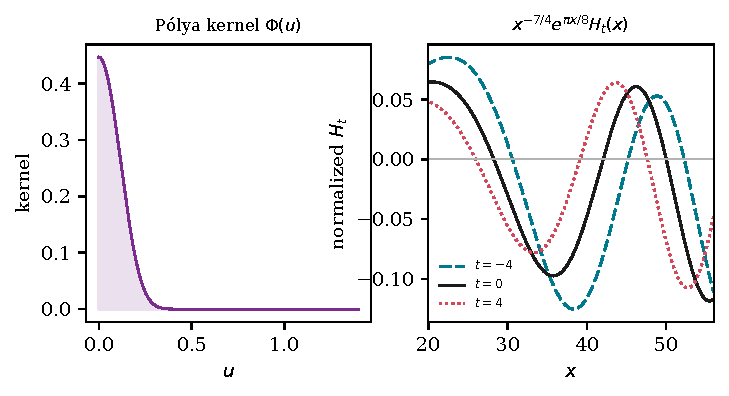
\includegraphics[width=\textwidth]{debruijn_newman}
\caption{Left, the P\'olya kernel $\Phi$. Right, $x^{-7/4}e^{\pi x/8}H_t(x)$ for $20\leq x\leq56$, computed by quadrature, for $t=-4$, $t=0$ (solid) and $t=4$, as marked in the legend. The factor $x^{-7/4}e^{\pi x/8}$ cancels the envelope $x^{7/4}e^{-\pi x/8}$ of $H_0$, which comes from the Gamma factor in $\xi$. The zeros of $H_0$ are twice the ordinates of the zeta zeros.}
\label{fig:debruijn_newman}
\end{figure}

The motion of the zeros has a formal description. If $H_t$ were a polynomial with simple zeros $z_k(t)$, differentiating $H_t(z_k(t)) = 0$ in $t$ and using the heat equation would give
\[
\dot z_k = \frac{\partial_z^2H_t(z_k)}{\partial_zH_t(z_k)} = 2\sum_{j\neq k}\frac{1}{z_k-z_j},
\]
a system of particles with logarithmic interaction, the same structure as Dyson's Brownian motion of Chapter~\ref{ch:brownian} without the noise. For entire functions of order one the sum must be interpreted with care, and Csordas, Smith and Varga~\cite{csv1994} made the description rigorous in a form sufficient to show that real zeros cannot collide and leave the real line under the backward flow. The proof of $\Lambda\geq0$ by Rodgers and Tao analyzes this dynamics, showing that if $\Lambda<0$ the zeros at $t = 0$ would be too regularly spaced, in contradiction with what is known about pair correlations of zeta zeros.

The analogy with Chapter~\ref{ch:nsinference} is formal. There, information about the initial condition of a dissipative equation is destroyed by forward evolution and must be recovered by backward inference, which is unstable at high frequencies. Here, the question is whether a structural property of an entire function, reality of zeros, survives backward evolution. The common structure is a Gaussian factor in Fourier space, $e^{-\nu|k|^2t}$ there and $e^{tu^2}$ here, and the analogy goes no further: the unknown there is an initial condition recovered from noisy data, and the function here is fixed.

\section{The Riemann hypothesis as a Lee Yang property}\label{sec:leeyangrh}

Let $X$ be a random variable with the symmetric density $\Phi(|u|)/\int_\R\Phi(|v|)\dd v$, which we call the P\'olya law. Its characteristic function is $\Xi(x/2)/\Xi(0)$, and its moment generating function is
\[
\E e^{sX} = \frac{\Xi(-is/2)}{\Xi(0)}.
\]
\begin{proposition}\label{prop:polyaleeyang}
The Riemann hypothesis holds if and only if the P\'olya law has the Lee Yang property of Chapter~\ref{ch:mixtures}.
\end{proposition}

\begin{proof}
The function $s\mapsto\E e^{sX} = \Xi(-is/2)/\Xi(0)$ is entire, because $\Phi(u)$ decays like $\exp(-\pi e^{4|u|})$ so that all exponential moments exist. Its zeros are the points $s$ with $\Xi(-is/2) = 0$, that is $s = 2ix$ with $\Xi(x) = 0$. Hence the zeros of the moment generating function are purely imaginary if and only if all zeros of $\Xi$ are real, which is the Riemann hypothesis since $\Xi(x) = \xi(\frac12+ix)$.
\end{proof} This is Newman's reformulation of 1976~\cite{newman1976}. In it, $e^{tu^2}$ is a Gaussian tilt of the single spin measure, and the de Bruijn Newman constant is the smallest $t$ for which the tilted P\'olya law has the Lee Yang property. Newman's motivation was a characterization of measures $\rho$ for which all ferromagnetic systems of spins with single spin law $\rho$ satisfy the Lee Yang theorem, and the Riemann hypothesis asks whether the P\'olya law belongs to a closely related class.

This reformulation explains why statistical mechanics enters number theory. Newman's theorem says that ferromagnetic couplings preserve the Lee Yang property. Multiplying a law with the Lee Yang property by $e^{bx^2}$ with $b\geq0$ preserves the property (Section~\ref{sec:ferromagnetic}, where it is derived from Newman's theorem by coupling to independent Ising spins). The Hubbard Stratonovich transformation writes this tilt as integrating out a Gaussian spin. It shows that if the tilted P\'olya law has the Lee Yang property at $t$, then it has the property at every larger $t$, which is Theorem~\ref{thm:polyadebruijn} again in the language of Chapter~\ref{ch:mixtures}. A proof of the Riemann hypothesis along these lines would exhibit the P\'olya law, which is the tilted law at $t = 0$, as a limit of ferromagnetic constructions. The companion volume~\cite{polsonh8} pursues a related route through Thorin measures: whether the reciprocal of $\Xi$, suitably normalized, is the Laplace transform of a generalized Gamma convolution, a positivity statement that is equivalent to the Riemann hypothesis.

\section{A Bayesian reading of the de Bruijn flow}

The family $e^{tu^2}\Phi(u)$, normalized, is an exponential family in the natural parameter $t$ with sufficient statistic $u^2$. Its characteristic functions are $H_t$, up to normalization. In the language of Chapter~\ref{ch:types}, varying $t$ is exponential tilting. The conditional limit theorem, which holds beyond finite alphabets under integrability conditions~\cite{csiszar1984}, identifies the tilted law as the limiting conditional law of one coordinate of a large P\'olya sample given its empirical second moment, and the integrability condition holds for every $t$ because $e^{tu^2}\Phi(u)$ is integrable. The de Bruijn flow is therefore the flow of conditional laws of a P\'olya distributed sample as the conditioning value of the empirical second moment increases. The Riemann hypothesis is the statement that the Lee Yang property holds at $t = 0$, which is conditioning on the typical value of the empirical second moment and returns the P\'olya law itself, and the theorem $\Lambda\geq0$ says that the property fails for every $t<0$, that is, for every conditioning value below the typical one. This reading suggests studying the constant through concentration and large deviation bounds for samples conditioned on their second moment.

\section{The Riemann hypothesis as a statement about Brownian motion}

Theorem~\ref{thm:bpy} of Biane, Pitman and Yor expresses $2\xi(s)$ as the Mellin transform $\E Y^s$ of a rescaled maximum of a Brownian excursion. The zeros of $\xi$ are the complex values of $s$ at which this Mellin transform vanishes. The Riemann hypothesis is therefore a statement about the law of a functional of Brownian motion: its Mellin transform vanishes only on the critical line. Several equivalent laws arise in the same paper, including the range of a Brownian bridge and sums of independent hitting times of Bessel processes, and the latter are generalized Gamma convolutions whose Thorin measures are explicit. The Brownian representation and the Thorin representation are two faces of the same object, and the passage between them is Kent's spectral theorem of Chapter~\ref{ch:brownian}.

\section{A computational strategy}

The Thorin measure of a GGC can be estimated from its Laplace transform by inverting the Stieltjes transform of the derivative of the Laplace exponent. For the reciprocal $\Xi$ problem, the Riemann hypothesis predicts a specific discrete Thorin measure supported on the squares of the zero ordinates. One can estimate the Thorin measure numerically from high precision evaluations of $\Xi$ and compare it with the measure predicted by the hypothesis, as a function of the truncation level. The predicted measure is purely atomic, and an estimate computed at a finite truncation level has a density or has its atoms elsewhere, so the two measures are mutually singular and their total variation distance would not tend to zero. The comparison must use a weak metric, such as the Wasserstein or L\'evy Prokhorov distance on windows, or compare Stieltjes transforms. Agreement to numerical precision on any finite window is not a proof, but the comparison isolates which positivity property would need to be proved, and it is the same kind of numerical certificate that the Yor identities of Chapter~\ref{ch:brownian} provide for their algorithms.

\section{Open problems}

We close with open problems drawn from the chapters of the book. Some are precise questions and some are programs, which we mark as such.

\begin{problem}[The inferential sixth problem]
This is a program, and its first task is to fix the regime. Consider hard spheres in the Boltzmann Grad limit with Gibbs initial data conditioned on a macroscopic density, velocity and temperature profile, observed through the hydrodynamic fields at a later time with noise of standard deviation $\sigma$. Find a relation between $\sigma$, the Knudsen number and the number of particles under which the deviation of the particle fields from the solution of the limiting fluid equations is small compared with $\sigma$, and prove under it a Bernstein von Mises theorem for smooth functionals of the initial macroscopic profile, with constants that do not depend on the number of particles.
\end{problem}

\begin{problem}[Poincar\'e]
Give quantitative versions of the method of arbitrary functions (Theorem~\ref{thm:arbitrary}) for mixed phase space systems such as H\'enon Heiles, where invariant tori and chaotic regions coexist, with rates in terms of the measure of the chaotic sea.
\end{problem}

\begin{problem}[Axioms]
Quantitative estimates for chaos and entropic chaos in Kac's model are known in several forms. Carlen, Carvalho, Le Roux, Loss and Villani~\cite{cclv2010} relate propagation of chaos to entropy and show, in particular, that the entropic rate of convergence to equilibrium can be arbitrarily slow. Hauray and Mischler~\cite{hauraymischler2014} compare Kac's chaos, entropic chaos and Fisher information chaos quantitatively, extend the estimates to measures on the Kac spheres, and treat mixtures in the sense of de Finetti, Hewitt and Savage. We do not know whether these estimates are optimal. Find the optimal rate, as a function of the marginal size $k$ and of $N$, in the finite de Finetti theorem for exchangeable laws on the sphere $S^{N-1}(\sqrt N)$ in relative entropy, with examples showing that it cannot be improved, and use it to prove a propagation of chaos theorem for Kac's model whose dependence on $N$ is optimal under explicit hypotheses on the initial law.
\end{problem}

\begin{problem}[Yor identities]
\label{prob:yor}
This is a program. Kent's theorem~\cite{kent1980} writes the hitting time of a level by a regular diffusion, started at a reflecting or entrance boundary, as a sum $\sum_nE_n/\lambda_n$ of independent exponential variables, where the $\lambda_n$ are eigenvalues of the generator. The part of the sum after the first $n$ terms is a generalized Gamma convolution with an explicit Thorin measure. Identify a class of regular diffusions for which this remainder can be sampled exactly with finite expected cost, prove that the resulting sampler is exact, and use it to build a library of exact samplers for Brownian functionals.
\end{problem}

\begin{problem}[Mixtures]
By Khintchine's theorem the P\'olya law of Section~\ref{sec:leeyangrh} is the law of $UZ$ with $U$ uniform on $[-1,1]$ and $Z\geq0$ independent of $U$. The law of $Z$ is not a generalized Gamma convolution, because $Z$ has finite exponential moments of every order and a nonconstant generalized Gamma convolution does not. The reciprocal of the moment generating function of $UZ$ at $2\sqrt\lambda$ is a different matter. It is $\Xi(0)/\Xi(i\sqrt\lambda) = \prod_n(1+\lambda/\gamma_n^2)^{-1}$, where $\pm\gamma_n$ are the zeros of $\Xi$, and it is the Laplace transform of a generalized Gamma convolution if and only if the Riemann hypothesis holds. In that case the Thorin measure is the sum of point masses at the $\gamma_n^2$. Conversely, the logarithmic derivative of the Laplace transform of a generalized Gamma convolution is analytic outside the negative half line, which forces all the $\gamma_n^2$ to be positive. Prove that this function is the Laplace transform of a generalized Gamma convolution by using the mixture representation $X = UZ$ and not the location of the zeros.
\end{problem}

\begin{problem}[Perelman]
Ni~\cite{ni2004} proved that the analog of the entropy $W$ of Theorem~\ref{thm:perelman_flat} for the linear heat equation on a Riemannian manifold is nonincreasing when the Ricci curvature is nonnegative. Extend the scale mixture proof of the monotonicity of $W$ (Theorem~\ref{thm:perelman_flat}) to Riemannian manifolds with nonnegative Ricci curvature, interpreting the Ricci term as a correction to the subordinated Brownian motion.
\end{problem}

\begin{problem}[Quantum]
Formulate a prior on Nelson's diffusions that does not itself impose the quantization condition, and identify data that determine the circulation of the drift around the nodes of the density, so that the posterior concentrates on drifts satisfying the quantization condition. Position statistics alone fix the density and, through the continuity equation, only the divergence of the current, so the data must carry more. A solution would give a Bayesian answer to Wallstrom's objection.
\end{problem}

\begin{problem}[Kinetic]
\label{prob:kinetic}
For the $N$ particle Kac walk with total collision rate $N$, let $H_N(F) = \int F\log F\dd\sigma_N$ be the relative entropy of a probability density $F$ with respect to the uniform law $\sigma_N$ on $S^{N-1}(\sqrt N)$, and let $D_N(F)$ be the rate at which $H_N$ decreases at time zero along the master equation started at $F$. Villani's argument~\cite{villani2003cercignani} gives $D_N(F)\geq2H_N(F)/(N-1)$. The best constant in this inequality tends to zero with $N$~\cite{cclv2010} and is at most $C_bN^{-1+2b}\log N$ for every $0<b<\frac16$, with $C_b$ depending only on $b$~\cite{einav2011}; Gao, Wang and Xia~\cite{gaowangxia2026} prove in a recent preprint that it equals $2/(N-1)$ for every $N\geq2$. The near extremal densities in these three works are conditioned products $F^f_N(v) = Z_N(f)^{-1}\prod_{i\leq N}f(v_i)$, where $f$ is a probability density on $\R$ and $Z_N(f) = \int\prod_{i\leq N}f(v_i)\,\sigma_N(\dd v)$. In the first two, $f$ is a mixture of two centered Gaussian densities, normalized to unit variance, with a fourth moment that is unbounded along the construction. Gao, Wang and Xia use two families: mixtures of two centered Gaussian densities, whose mixing law has two atoms and so is not a generalized Gamma convolution, and $f$ proportional to $(a+v^2)^{-q}$, with $a\to0$ and then $q\to\frac12$ at fixed $N$. The latter $f$ is a rescaled Student law with $2q-1$ degrees of freedom, hence a normal scale mixture whose inverse Gamma mixing law is a generalized Gamma convolution (Appendix~\ref{app:levy}); its variance tends to zero or is infinite, and the energy concentrates on one particle. Without moment conditions, restricting $f$ to such mixtures therefore does not improve the constant $2/(N-1)$. Fix $M>3$, and let $\mathcal G_M$ be the set of bounded densities $f$ that are normal scale mixtures with generalized Gamma convolution mixing law and satisfy $\int v^2f(v)\dd v = 1$ and $\int v^4f(v)\dd v\leq M$. Decide whether there is $\lambda>0$, depending only on $M$, such that $D_N(F^f_N)\geq\lambda H_N(F^f_N)$ for every $N\geq2$ and every $f\in\mathcal G_M$. Carlen, Carvalho, Le Roux, Loss and Villani~\cite{cclv2010} raise the question whether a fixed bound on the fourth moment gives a bound of this kind without the condition on the mixing law, and Carlen, Carvalho and Einav~\cite{carlencarvalhoeinav2018} prove inequalities of the weaker form $D_N(F)/N\geq C(H_N(F)/N)^{1+\varepsilon}$, with $C$ independent of $N$, for data with bounded moments that satisfy a quantitative form of chaos.
\end{problem}

\begin{problem}[Hydrodynamics]
Derive the incompressible Navier Stokes Fourier system from hard sphere dynamics in a bounded domain with Maxwell reflection boundary conditions, identifying the boundary layers in the limit. The torus in dimensions two and three is treated in the preprint~\cite{denghanima2025}, and the problem is the extension to domains with boundary.
\end{problem}

\begin{problem}[Inference]
\label{prob:inference}
Konen and Nickl~\cite{konennickl2026} prove a functional Bernstein von Mises theorem for the posterior of the trajectory of the two dimensional Navier Stokes equations on the torus, with root $N$ consistent prediction of future states in the supremum norm, for a Gaussian prior on the initial condition and $N$ noisy observations at uniformly random points of space and time. We know of no corresponding result for sensors at fixed locations or for other priors. Determine the posterior contraction rate for the initial vorticity from noisy point observations at a fixed array of sensors and times, in terms of the number of sensors, the number of times and the noise level, and identify the functionals of the initial vorticity that admit a Bernstein von Mises theorem. A companion question is whether the posterior of the initial vorticity can be computed in time polynomial in the data size and the dimension; Section~\ref{sec:gradstab} records what is known.
\end{problem}

\begin{problem}[Blowup]
Fix a finite horizon and a computable blowup criterion, for example that a norm of the solution of a Galerkin truncation of the equations exceeds a threshold before the horizon. Construct a prior on initial data and forcing for three dimensional Navier Stokes and a sequence of numerical solvers such that the posterior probability of this event is consistent, that is, converges to its true value as the resolution and the amount of data increase, and quantify how the event approximates finite time blowup of the exact solution. Consistency for the blowup of the exact solution itself, under either hypothesis, would require deciding the regularity of the data near the truth, which is the regularity problem.
\end{problem}

\begin{problem}[Onsager]
This is a program. At finite Reynolds number the velocity field is smooth, so a H\"older exponent has to be defined through an inertial range statement, such as the scaling $S_p(\ell)\propto\ell^{\zeta_p}$ of the structure functions. Develop a joint posterior for the exponents $\zeta_p$ and the inertial range from measured velocity increments, and use it to ask whether laboratory and numerical data concentrate at, above or below the exponents $\zeta_p = p/3$ of Kolmogorov and Onsager.
\end{problem}

\begin{problem}[Phase transitions]
Chapter~\ref{ch:spins} records what is known for the planted clique problem with a known clique size $k$ in the graph $G(n,\frac12)$: approximate message passing succeeds for $k\geq(1+\varepsilon)\sqrt{n/e}$, and from a suitable starting state the Metropolis process cannot find a planted clique of size $k = n^{1/2-\varepsilon}$ in polynomial time. Take as samplers of the posterior over clique locations either Glauber dynamics on vertex sets of size $k$, or Langevin dynamics for a continuous relaxation of the clique indicator, in both cases initialized from the prior. Determine whether such samplers have a computational phase transition at $k = \sqrt{n/e}$, in the sense that they succeed in polynomial time above $(1+\varepsilon)\sqrt{n/e}$ and fail below $(1-\varepsilon)\sqrt{n/e}$.
\end{problem}

\begin{problem}[Transport]
Prove convergence rates for generative Bayesian computation via learned Schr\"odinger bridges in terms of the entropic regularization, the number of simulations and the smoothness of the posterior. Rates in the sample size are known for the entropic optimal transport cost estimated from samples, by Genevay, Chizat, Bach, Cuturi and Peyr\'e~\cite{genevay2019} and by Mena and Niles Weed~\cite{menaniles2019}. The problem concerns the learned bridge as an estimator of the posterior.
\end{problem}

\begin{problem}[Thermodynamics of inference]
The Landauer bound (Theorem~\ref{thm:landauer}) bounds the heat dissipated by a physical process in terms of the entropy removed, and the Sagawa Ueda inequality of Chapter~\ref{ch:kolmogorov} bounds the work in terms of the mutual information acquired. For a Bayesian update from a prior $\mu_0$ to the posterior $\mu_y$, prove a lower bound on the heat dissipated by any physical implementation in terms of $\KL(\mu_y\|\mu_0)$ and the information erased, and compare it with the dissipation of Langevin samplers.
\end{problem}

\begin{problem}[The bridge]
This is a program whose goal is the Riemann hypothesis, which is equivalent to $\Lambda\leq0$. Newman's theorem (Chapter~\ref{ch:mixtures}) produces laws with the Lee Yang property from independent single spin laws with that property by ferromagnetic couplings. Decide whether the P\'olya law is the weak limit of a sequence of laws of random variables $X_n$ obtained by such constructions from Ising spins and uniform laws, with $\sup_n\E e^{c|X_n|}<\infty$ for every $c>0$, which is the control that carries the Lee Yang property to the limit by Hurwitz's theorem. A construction would prove the Riemann hypothesis by Proposition~\ref{prop:polyaleeyang}, and a proof that none exists would show that this route to the hypothesis is closed.
\end{problem}

\section{Conclusion}

Hilbert asked for the passage from atoms to continua with full rigor. A century and a quarter later the passage has been announced for a rarefied gas of hard spheres on the torus by Deng, Hani and Ma in two preprints~\cite{denghanima2024,denghanima2025}, building on the work of Lanford, Bardos, Golse, Levermore and Saint Raymond. Kolmogorov supplied the probability, Poincar\'e the warnings and the first rigorous mechanism of chance, Boltzmann the vision. The inverse passage, from continua back to the states that produced them, is younger and less complete. It rests on the same mathematics and it inherits the same limitations at the boundary of regularity. We have argued that Bayesian computation is the natural language for that inverse passage and that inference is itself a problem of statistical mechanics. If the argument is right, Hilbert's sixth problem is not closed; it has acquired a second half.

We do not claim a proof of the Riemann hypothesis, of the global regularity of the Navier Stokes equations, or of any of the open problems above. What we claim is structural. The mathematics that Hilbert's sixth problem required, probability measures on spaces of trajectories, entropy, transport and the heat equation, is also the mathematics in which the eighth problem has its probabilistic formulations, and the mathematics in which Bayesian computation is carried out. Several of the open problems, among them the last, ask for theorems about the heat equation, its backward flow and the measures it transports. The sixth problem taught that such theorems are about limits and about the measures on initial conditions with respect to which the limits hold. The inferential reading taught that those measures can be learned. Whether the same lessons apply to the zeros of $\Xi$ is, for now, an open question.

\section*{Exercises}
\begin{enumerate}
\item Justify differentiation under the integral sign in $\partial_tH_t = -\partial_z^2H_t$.
\item Show that $H_0(z) = \frac18\Xi(z/2)$.
\item For a real polynomial with simple real zeros evolving by $\partial_tp = -p''$, derive $\dot z_k = 2\sum_{j\neq k}(z_k-z_j)^{-1}$.
\item Show that $e^{-\lambda D^2}(z^2-1) = z^2-1-2\lambda$, and determine the values of $\lambda$, positive or negative, for which the zeros are real.
\item Express $\E Y^2$ and $\E Y^4$ in the Biane, Pitman and Yor identity through values of $\xi$, and evaluate them numerically.
\end{enumerate}


\section*{Notes}

De Bruijn~\cite{debruijn1950} proved a zero free strip bound, Theorem~13 of that paper: if $H_{t_0}$ has no zeros with $|\Im z|>y_0$, then for $t>t_0$ the function $H_t$ has none with $|\Im z|>\sqrt{\max(y_0^2-2(t-t_0),0)}$. The zeros of $H_0$ satisfy $|\Im z|<1$, so $t_0 = 0$ and $y_0 = 1$ give $\Lambda\leq\frac12$. The monotonicity in $t$ follows from results of P\'olya~\cite{polya1927}. Platt and Trudgian~\cite{platttrudgian2021} obtain $\Lambda\leq0.2$ by combining a conditional bound of the Polymath paper~\cite{polymath2019}, its Table~1, with their verification of the Riemann hypothesis up to height $3\cdot10^{12}$.
